\begin{mainquestion}{hfpulse}{High-Frequency Pulse Amplifier}

The figure below shows a scheme for coupling and amplifying a high-frequency pulse signal. The circuit uses two MOSFETs whose details are not shown and a 50-$\Omega$ coaxial cable. For proper operation (with no signal reflections coming back down the cable), transistor $Q_{2}$ is required to present a 50-$\Omega$ resistance to the cable. That is, the input resistance for $Q_{2}$ is \qty{50}{\ohm}.

\begin{center}
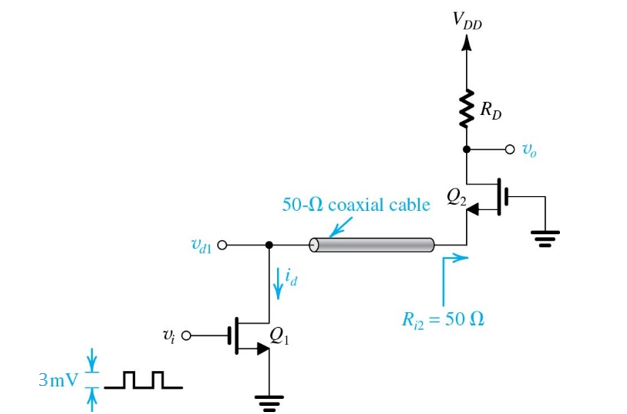
\includegraphics[width=4.5in]{pic6.png}
\end{center}

\begin{partquestion}{amplifiertypes}{In what type of amplifier is $Q_{1}$ operating? In what type of amplifier is $Q_{2}$ operating?}
\begin{answer}
$Q_{1}$ is a common source amplifier, with the input at the gate and the output at the drain. $Q_{2}$ is a common gate amplifier, with the input at the source and the output at the drain.
\end{answer}
\end{partquestion}

\begin{partquestion}{gm2}{What is $\mathbf{g}_{\mathbf{m2}}$?}
\begin{answer}
The input resistance to a common gate (CG) amplifier is $R_{\text{in}} = 1/g_{m} = \qty{50}{\ohm}$, so $g_{m2} = \qty{0.02}{\siemens}$.
\end{answer}
\end{partquestion}

\begin{partquestion}{currentpulse}{If $Q_{1}$ and $Q_{2}$ are biased (operating) at the same point, what is the amplitude of the high-frequency current pulses in the drain of $Q_{1}$?}
\begin{answer}
Note that the current flowing through $Q_2$ all flows through $Q_1$. If the two transistors have the same current and the same overdrive voltage, then $g_{m1} = g_{m2} = \qty{0.02}{\siemens}$. For an input amplitude of 3 mV, the output current amplitude is:

\[
0.003 \cdot 0.02 = \qty{0.06}{\milli\ampere}.
\]

Note that because the CS is an inverting amplifier, the pulses will be negative.
\end{answer}
\end{partquestion}

\begin{partquestion}{voltagepulse}{What is the amplitude of the high-frequency voltage pulses at the drain of $Q_{1}$?}
\begin{answer}
Assuming $r_{o}$ is large enough to be ignored, the pulse amplitude is:

\[
g_{m} R v_{i} = (0.02)(50)(\qty{3}{\milli\volt}) = \qty{3}{\milli\volt}.
\]

Again, the pulses will be negative due to the inverting amplifier.
\end{answer}
\end{partquestion}

\begin{partquestion}{rdvalue}{What is the value of $R_D$ required to provide 1-volt pulses at the drain of $Q_{2}$?}
\begin{answer}
The voltage gain of the CG amplifier is $g_{m}R_{D}$, and if we have 3 mV amplitude pulses at the input to $Q_2$ then (again when $r_{o}$ is sufficiently large) we have amplitude:

\begin{align*}
    R_D &= \frac{1}{g_m(0.003)} \\
    &= \frac{1}{(0.02)(0.003)} \\
    &= \qty{16.67}{\kilo\ohm}
\end{align*}

Shoot, we might as well just round up again to \qty{17}{\kilo\ohm}, since we are on a roll!

\end{answer}
\end{partquestion}

\end{mainquestion}
